
% --------------------------------------------------------------
\begin{chapter}{Probability Elicitation: Weibull \label{Chap:elic-weib}}
The Athena simulator \cite{Zit13, Zit16} has a large number of input parameters which, broadly, can be divided into two classes. We have ``known'' inputs which, in some sense, are model assumptions or parameters relating to a decision. For instance, this might reflect the location of a future windfarm, the number of turbines the windfarm has or anything else that would be known with certainty. The second set would be the unknown parameters which are to be elicited for uncertainty analyses. For instance, this might be the expected lifetimes of components in the windfarm or the time taken for repairs of failed components; these may be a function of the decision taken by the DM. \\

\begin{figure}
	\centering
	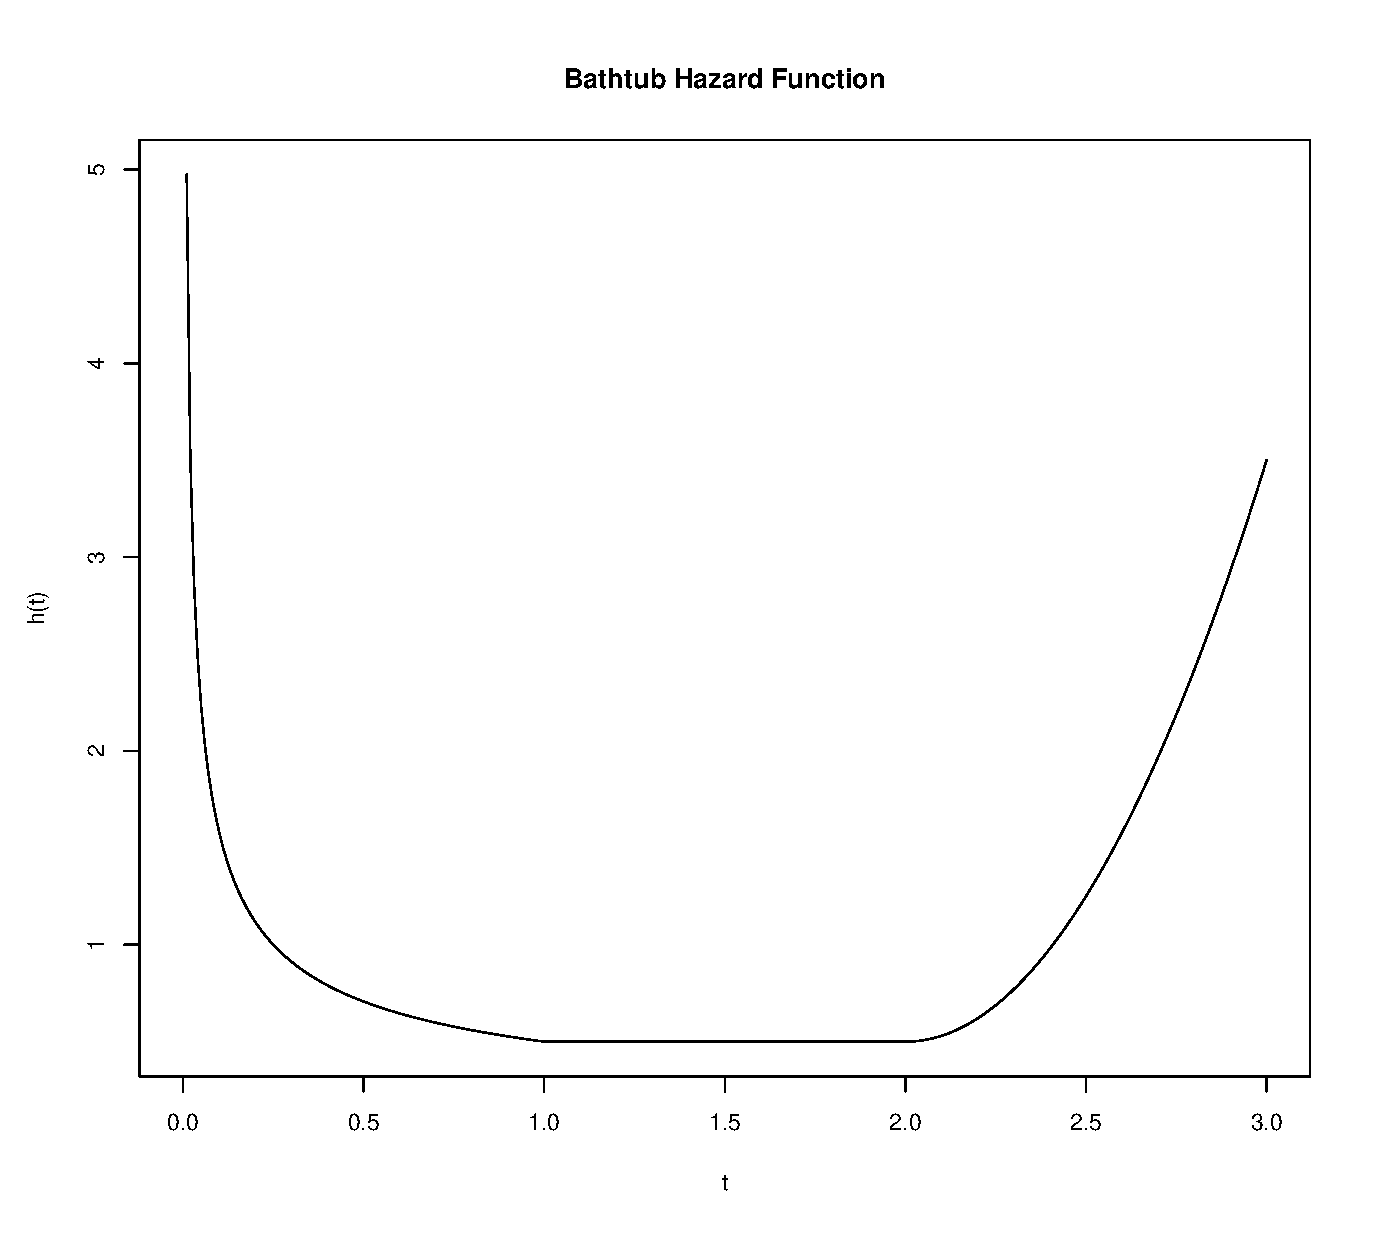
\includegraphics[width = 0.8\textwidth]{fig-elic/bathtub-hazard.eps}
	\caption{Bathtub shaped hazard function.}
	\label{Fig:bathtub}
\end{figure}
For a general overview of elicitation see \citep{Garthwaite05, Ohagan06}. In this chapter we focus on the elicitation for lifetimes of components in the windfarm (mainly that of the key ``subassemblies'' of a windfarm, which are the major components of a single wind turbine). The windfarm components are assumed to follow Weibull distributions; this is one of the key assumptions of the windfarm model. \cite{Ren13} discuss a method for elicitation of (human) lifetimes which are assumed Weibull; this can be applied to the lifetimes of mechanical components. However, adaptations are made to Ren $\&$ Oakley's method to take into account the shape of hazard functions of components. In \cite{Wang02} it is explained that the hazard function of a component can be split into three phases, and follows a ``bathtub'' shape (see \Cref{Fig:bathtub}). If we assume that the length of each phase ($T$) is Weibull, i.e. $T \sim Weibull(\lambda, \kappa)$ where $\lambda > 0$ is the scale parameter and $\kappa > 0$ the shape parameter, the three phases are as follows:
\begin{itemize}
	\item Early life, infant mortality present so $\kappa <1$
	\item Useful life (after early life), here $\kappa = 1$
	\item Degradation period (after useful life) $\kappa > 1$.
\end{itemize}
Note that we are using the form of the Weibull distribution with the following pdf:
\begin{equation}
	f(t) = \frac{\kappa}{\lambda} \left( \frac{t}{\lambda}\right)^{\kappa - 1} \exp \big\{ (t/ \lambda)^\kappa \big\}, \quad t \geq 0.
\end{equation}
To take this physical constraint into account, we have to condition on $\kappa$ being within the relevant regions of the parameter space for each phase of subassembly life. The useful life is simple since $\kappa = 1$ reduces to an Exponential distribution. When $\kappa =  1$ this implies that all failures are from an external source, e.g. catastrophic weather events. However, for the other two cases care must be taken in the elicitation procedure to prevent the expert from giving inconsistent probability statements (e.g. allowing $\kappa<1$ to have non-negligible probability in the third phase). This is done by asking the experts to use interval bisection, where the expert is asked to split the possible parameter space into equally likely regions. However, for elicitation we must relate the parameters of the distribution to observable quantities. Here we can use

\begin{align*}
	\pi_0 &= \p(T > t_0)\\
		&= \exp \{ -(t_0/ \lambda)^\kappa \}\\
	\delta &= \p(T>t_1 | T > t_0)\\
	& = \exp\{ (t_0/\lambda)^\kappa - (t_1/ \lambda)^\kappa \} 
\end{align*}
we can then deduce that
\begin{equation}
\dfrac{\log(\pi_0)}{\log(\pi_0 \delta)} = \bigg( \dfrac{t_0}{t_1}\bigg) ^\kappa \label{Eq:kappa-exponent}
\end{equation}
and hence, 
\begin{equation}
\kappa =  \dfrac{\log \bigg\{ \dfrac{\log(\pi_0)}{\log(\pi_0 \delta)} \bigg\}}{\log \bigg\{ \dfrac{t_0}{t_1}\bigg\}} \label{Eq:kappa}
\end{equation}
\begin{equation}
\lambda = t_0 \big( - \log \pi_0\big)^{-1/\kappa}. \label{Eq:lambda}
\end{equation}

It can easily be shown that if $\kappa > 1$ then it must be the case that 
\begin{equation}
	\pi_0 ^{t_1 - t_0} > \delta^{t_0}. \label{Eq:pi0-delta}
\end{equation}
This implies the probability of survival decreases quickly with time. Hence in order to elicit \textit{coherent} summaries from the experts we must structure the elicitation carefully. One way to do this is by first eliciting $\pi_0$ and then eliciting $\delta$ conditional on a particular value of $\pi_0$. So if we take $t_1 = 2$, $t_0 = 1$ then we might ask the expert(s):\\\\

\textit{``Split the interval $(0, 1)$ into two intervals such that the probability a component is still functioning properly at time $t_0$ is equally likely to be in either interval.''}\\\\

We can then ask the expert to split these intervals again to obtain the median and lower/upper quartiles for $\pi_0$. We can then use least squares to fit these summaries to a beta distribution; a natural choice for proportions. To obtain $\delta$ subject to $\kappa>1$ we can ask the expert to split the interval $(0, p_0)$ into three equally likely intervals to give a medial and lower/upper quartiles. Here, $p_0$ is the value of $\pi_0$ that the expert thinks is plausible; for example, their upper quartile for $\pi_0$. We could then fit these quantiles to a scaled beta distribution defined on the interval $(0, p_0)$. This induces a hierarchical prior of the form
\begin{align}
	\pi_0 &\sim Beta(a_0, b_0) \\
	\delta | \pi_0 & \sim ScBeta_{(0, \pi_0)} (a_1, b_1)
\end{align}
Where $Y \sim ScBeta_{(l ,u)}(a, b)$ is the distribution obtained from the transformation 
\begin{equation}
	Y = l + (u - l)X
\end{equation}
where $X \sim Beta(a, b)$. \\\\
 We can then draw many samples of $(\pi_0, \delta)$ and use to obtain many samples of $(\lambda, \kappa)$. Not having the distribution of $(\lambda, \kappa)$ in closed form is not likely to be problematic since at some point we are going to evaluate the simulator/emulator at many samples to propagate this uncertainty to understand the induced uncertainty on model outputs.\\\\

We could repeat the above process for each component of the windfarm of interest, which would give us independent pairs $(\lambda_i, \kappa_i)$ for components $i = 1, \ldots, N$. The experts however might believe that component lifetimes are statistically dependent (not physically dependent). One such way to induce this dependence is to allow components to share a value of $\kappa$, but possibly have different values of $\lambda$. If we have $n$ components which the expert believes have dependent lifetimes, then we could elicit pairs of $(\pi_{0,i}, \delta_i)$ for each component and then minimise the following objective function to find an ``agreed'' value of $\kappa$ for the set of components with dependent lifetimes
\begin{equation}
h(\kappa) = \sum_{i = 1}^n \left\{\kappa - \dfrac{\log \bigg[ \dfrac{\log(\pi_{0,i})}{\log(\pi_{0,i} \delta_i)} \bigg]}{\log \bigg[ \dfrac{t_0}{t_1}\bigg]} \right\}^2 .\label{Eq:optim-fn}
\end{equation}


 For instance, splitting into four regions gives us the median and lower and upper quartiles, but there is evidence to suggest splitting into three regions (tertiles) may help the experts give more reliable probability statements (\cite{Ohagan06} mention that frequently experts can be very over confident in their beliefs).\\\\
 
 We will now briefly show how this would work with an example. Suppose we had an elicitation with some experts and we had $N = 2$ dependent subassemblies labelled $1$ and $2$, with $t_0 = 1$ and $t_1 = 2$. We might first ask about subassembly $1$ and then subassembly $2$. The expert might give us prior information which leads to  $\pi_{0,1} \sim Beta(24.68, 3.198)$, $\delta_1 | \pi_{0,1} \sim ScBeta_{(0, \pi_{0,1})}(19.53, 3.11)$, $\pi_{0,2} \sim Beta(1383.4, 28.72)$ and finally $\delta_1 | \pi_{0,2} \sim ScBeta_{(0, \pi_{0,2})}(93.19, 8.534)$.
 \begin{figure}
 	\centering
 	\includegraphics[width = 0.6\textwidth]{fig-elic/pi-delta-plot.eps}
 	\caption{Pairwise plot of the elicited joint distribution of lifetimes.}
 	\label{Fig:pi-delta1}
 \end{figure}
 In \Cref{Fig:pi-delta1} we see most the striking relationship is that between the $\pi_{0,i}$ and the corresponding $\delta_i$, with the hard cut-off being induced by the scaled Beta distribution over $\delta_i | \pi_{0,i}$.
 \begin{figure}
 	\centering
 	\includegraphics[width = 0.6\textwidth]{fig-elic/lambda-kappa.eps}
 	\caption{Pairwise plot of the elicited joint distribution of Weibull parameters.}
 	\label{Fig:lambda-kappa1}
 \end{figure}
 Then in \Cref{Fig:lambda-kappa1} we see how the expert's beliefs about specific lifetimes translate into statements about the corresponding Weibull parameters. Crucially, we see that $\kappa\leq 1$ is given zero density thus ensuring that we observe ageing of components in the windfarm.\\\\
 
 The above lays out how to elicit for $\kappa >1$, the process is similar for $\kappa<1$ but when $\kappa<1$ we have $\pi_0 < \delta$ (for the same choices of $t_0$ and $t_1$). When $\kappa = 1$ we would have $\pi_0 = \delta$.
 %% insert plots
\end{chapter}
